\documentclass[conference]{IEEEtran}

% Required packages
\usepackage{cite}
\usepackage{amsmath,amssymb,amsfonts}
\usepackage{algorithmic}
\usepackage{graphicx}
\usepackage{textcomp}
\usepackage{xcolor}
\usepackage{booktabs}
\usepackage{tikz}
\usepackage{tikz-timing}

% TikZ libraries
\usetikzlibrary{shapes.geometric, arrows.meta, positioning, fit, calc, decorations.pathreplacing}

\begin{document}

\title{Out-of-Order RISC-V Processor: Design, Implementation, and Evaluation}

\author{
    \IEEEauthorblockN{[Team member names]}
    \IEEEauthorblockA{EECS 4340, Spring 2026 \\
    Columbia University}
}

\maketitle

\begin{abstract}
% [Paste from draft.md §Abstract]
\end{abstract}

\section{Introduction}
% [Paste from draft.md §I]

\section{Background and Constraints}
% [Paste from draft.md §II]

\section{Pipeline Architecture}
% [Paste from draft.md §III]

% Figure 1 — Top-level pipeline block diagram (after the dataflow paragraph)
\begin{figure}[t]
    \centering
    % Figure 1 -- Top-level pipeline block diagram
% Five vertical bands: Fetch | Decode | Dispatch/Rename | Issue/Execute | Commit
% Uses only TikZ libraries already loaded in main.tex:
%   shapes.geometric, arrows.meta, positioning, fit
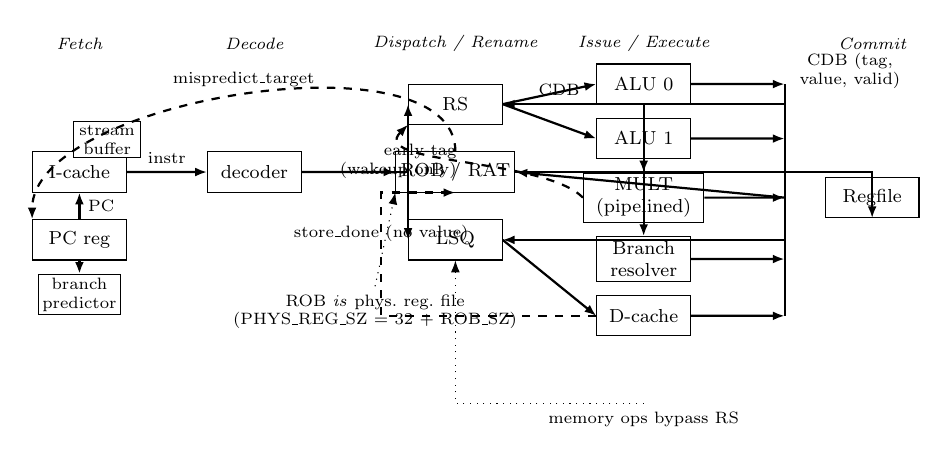
\begin{tikzpicture}[
    scale=0.85, transform shape,
    every node/.style={color=black, font=\footnotesize},
    box/.style={draw, rectangle, minimum height=6mm, minimum width=14mm,
                align=center, inner sep=2pt, color=black},
    smallbox/.style={draw, rectangle, minimum height=4.5mm, minimum width=10mm,
                     align=center, inner sep=1.5pt, font=\scriptsize, color=black},
    bandlabel/.style={font=\scriptsize\itshape, color=black},
    annot/.style={font=\scriptsize, color=black, align=center},
    arrow/.style={-{Latex[length=1.5mm]}, color=black, thick},
    sideband/.style={-{Latex[length=1.5mm]}, color=black, dashed, thick},
    >={Latex[length=1.5mm]}
]

% --- Fetch band ---
\node[box] (pc) at (0, 0) {PC reg};
\node[smallbox, below=2mm of pc] (bp) {branch\\predictor};
\node[box, above=4mm of pc] (ic) {I-cache};
\node[smallbox, above right=-1mm and -8mm of ic, fill=white] (sb) {stream\\buffer};

% --- Decode band ---
\node[box, right=12mm of ic] (dec) {decoder};

% --- Dispatch band ---
\node[box, right=14mm of dec] (rob) {ROB / RAT};
\node[box, above=4mm of rob] (rs) {RS};
\node[box, below=4mm of rob] (lsq) {LSQ};

% --- Issue/Execute band ---
\node[box, right=14mm of rs, yshift=3mm] (alu0) {ALU 0};
\node[box, below=2mm of alu0] (alu1) {ALU 1};
\node[box, below=2mm of alu1, minimum width=18mm] (mult) {MULT\\(pipelined)};
\node[box, below=2mm of mult] (br) {Branch\\resolver};
\node[box, below=2mm of br] (dc) {D-cache};

% --- Commit band ---
\node[box, right=18mm of mult] (rf) {Regfile};

% --- Band labels (above the diagram) ---
\node[bandlabel, above=14mm of ic] (lblF) {Fetch};
\node[bandlabel] at (dec |- lblF) {Decode};
\node[bandlabel] at (rob |- lblF) {Dispatch / Rename};
\node[bandlabel] at (alu0 |- lblF) {Issue / Execute};
\node[bandlabel] at (rf  |- lblF) {Commit};

% --- Solid arrows (datapath) ---
% PC bus
\draw[arrow] (pc.north) -- node[right, font=\scriptsize] {PC} (ic.south);
\draw[arrow] (pc.south) -- (bp.north);
% I-cache to decoder (instruction bus)
\draw[arrow] (ic.east) -- node[above, font=\scriptsize] {instr} (dec.west);

% Decoder to dispatch fork (ROB, RS, LSQ)
\draw[arrow] (dec.east) -- (rob.west);
\draw[arrow] (dec.east) -| (rs.west);
\draw[arrow] (dec.east) -| (lsq.west);

% Dispatch to execute units
\draw[arrow] (rs.east) -- (alu0.west);
\draw[arrow] (rs.east) -- (alu1.west);
\draw[arrow] (rs.east) -| (mult.north);
\draw[arrow] (rs.east) -| (br.north);
\draw[arrow] (lsq.east) -- (dc.west);

% Commit: ROB to Regfile
\draw[arrow] (rob.east) -| (rf.south);

% --- CDB (single bus from execute back to RS, ROB, LSQ) ---
% A vertical spine sits to the right of all execute units; each unit feeds it,
% and horizontals from the spine return to RS / ROB / LSQ.
\coordinate (spineTop)  at (alu0.east -| rf.west);
\coordinate (spineMid)  at (mult.east -| rf.west);
\coordinate (spineBot)  at (dc.east   -| rf.west);
% Move the spine slightly left of Regfile so we don't collide with it.
\coordinate (spineTopL) at ([xshift=-6mm] spineTop);
\coordinate (spineMidL) at ([xshift=-6mm] spineMid);
\coordinate (spineBotL) at ([xshift=-6mm] spineBot);
\coordinate (spineALU1) at (alu1.east -| spineTopL);
\coordinate (spineBR)   at (br.east   -| spineTopL);
% Per-unit feeders into the spine
\draw[arrow] (alu0.east) -- (spineTopL);
\draw[arrow] (alu1.east) -- (spineALU1);
\draw[arrow] (mult.east) -- (spineMidL);
\draw[arrow] (br.east)   -- (spineBR);
\draw[arrow] (dc.east)   -- (spineBotL);
% Vertical spine
\draw[thick] (spineTopL) -- (spineBotL);
% Returns to RS, ROB, LSQ (these go back to the left, so we route below RS / above LSQ)
\draw[arrow] (spineTopL) |- node[above, pos=0.9, font=\scriptsize] {CDB} (rs.east);
\draw[arrow] (spineMidL) -- (rob.east);
\draw[arrow] (spineBotL) |- (lsq.east);

% CDB label
\node[annot, right=1mm of spineTopL, yshift=2mm] {CDB (tag,\\value, valid)};

% --- Dashed sideband: early-tag from MULT to RS ---
\draw[sideband] (mult.west) .. controls +(-6mm,6mm) and +(-6mm,-6mm) ..
    node[left, pos=0.5, font=\scriptsize, align=right] {early-tag\\(wakeup only)} (rs.south west);

% --- Dashed sideband: store_done from D-cache to ROB ---
\draw[sideband] (dc.west) -| ([xshift=-4mm] lsq.west) |-
    node[below, pos=0.25, font=\scriptsize] {store\_done (no value)} (rob.south);

% --- Dashed mispredict redirect: ROB to PC reg, curved feedback above the bands ---
\draw[sideband] (rob.north) .. controls +(0,18mm) and +(0,18mm) ..
    node[above, midway, font=\scriptsize] {mispredict\_target} (pc.north west);

% --- Annotations ---
\node[annot, below=10mm of dc] (annot1) {memory ops bypass RS};
\draw[->, color=black, dotted] (annot1.north) -| (lsq.south);

\node[annot, below=14mm of rob, xshift=-12mm] (annot2)
    {ROB \emph{is} phys.\ reg.\ file\\(PHYS\_REG\_SZ = 32 + ROB\_SZ)};
\draw[->, color=black, dotted] (annot2.north) -- (rob.south west);

\end{tikzpicture}

    \caption{Top-level pipeline. Fetch and commit are in-order; issue and execute are out-of-order. The Reorder Buffer doubles as the physical register file, and a single Common Data Bus is the only result-broadcast network in the base configuration.}
    \label{fig:pipeline}
\end{figure}

\section{Base Implementation Details}
% [Paste from draft.md §IV]

\section{Advanced Features}
% [Paste from draft.md §V opener]

% Table I — Spec-compliance feature mapping (placeholder; see Task 25)
% [TABLE I goes here — migrated in Task 25]

\subsection{2-way Superscalar}
% [Paste from draft.md §V.A]

\subsection{Early Tag Broadcast}
% [Paste from draft.md §V.B]

% Figure 5 — Early-tag-broadcast timing
\begin{figure}[t]
    \centering
    % Figure 5 - Early-tag-broadcast timing diagram.
%
% Cycles 0..9 along the x-axis.  Cycle 0 = MULT enters stage 0; the
% early-tag sideband fires.  The dependent RS entry's src_ready is
% registered, so it settles at cycle 1.  The MULT result reaches the CDB at
% cycle 7 and the dependent RS issues that same cycle via the CDB-bypass
% mux.  Without ETB the dependent issue would be deferred to cycle 8.
%
% Implemented as a hand-built TikZ waveform (rectangular pulses) for
% predictable layout independent of tikz-timing version quirks.

\usetikzlibrary{calc, decorations.pathreplacing}

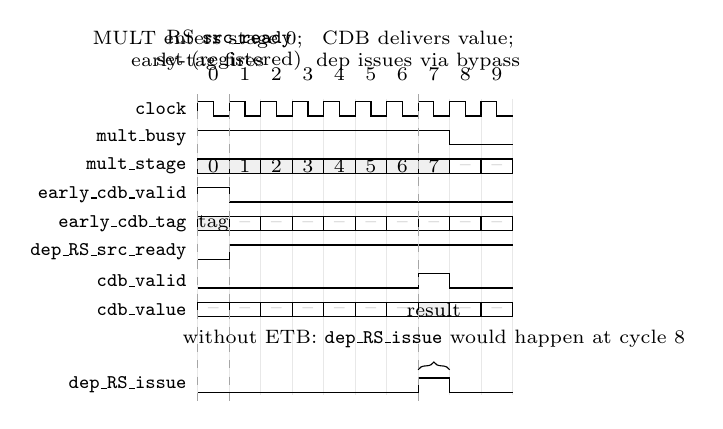
\begin{tikzpicture}[
    font=\scriptsize,
    x=4mm,                  % one TikZ unit = one cycle width
    y=2.6mm,                % one TikZ unit = one row height
    rowlabel/.style = {anchor=east, font=\scriptsize\ttfamily,
                       inner sep=1pt, xshift=-1mm},
    wave/.style     = {line width=0.45pt, line cap=square,
                       line join=miter, color=black},
    guide/.style    = {dashed, gray!70, thin},
    glab/.style     = {font=\scriptsize, align=center, inner sep=1pt}
]

% --- Geometry -----------------------------------------------------------
% Total width spans cycles 0..9 (10 cycles).  Each row is centred at its
% own integer y; the waveform vertical excursion is +/- 0.35.
\def\Ncyc{10}
\def\hi{0.35}
\def\lo{-0.35}

% Row y-positions (top to bottom).  Extra gap before the dep_RS_issue row
% leaves room for the "without ETB" bracket directly above it.
\def\yClk   { 0}
\def\yBusy  {-1.4}
\def\yStg   {-2.8}
\def\yEv    {-4.2}
\def\yEt    {-5.6}
\def\ySr    {-7.0}
\def\yCv    {-8.4}
\def\yCval  {-9.8}
\def\yDi    {-13.5}

% --- Row labels --------------------------------------------------------
\node[rowlabel] at (0, \yClk)  {clock};
\node[rowlabel] at (0, \yBusy) {mult\_busy};
\node[rowlabel] at (0, \yStg)  {mult\_stage};
\node[rowlabel] at (0, \yEv)   {early\_cdb\_valid};
\node[rowlabel] at (0, \yEt)   {early\_cdb\_tag};
\node[rowlabel] at (0, \ySr)   {dep\_RS\_src\_ready};
\node[rowlabel] at (0, \yCv)   {cdb\_valid};
\node[rowlabel] at (0, \yCval) {cdb\_value};
\node[rowlabel] at (0, \yDi)   {dep\_RS\_issue};

% --- Cycle column labels (top) ----------------------------------------
\foreach \c in {0,...,9} {%
    \node[font=\scriptsize, anchor=south]
        at (\c+0.5, \yClk + 0.9) {\c};
}

% --- Light cycle gridlines (very faint) -------------------------------
\foreach \c in {0,1,2,3,4,5,6,7,8,9,10} {%
    \draw[gray!18, line width=0.2pt] (\c, \yClk + 0.5) -- (\c, \yDi - 0.5);
}

% =====================================================================
% clock - square wave: high for first half-cycle, low for second.
% =====================================================================
\draw[wave]
    (0, \yClk + \lo)
    \foreach \c in {0,...,9} {%
        -- (\c,         \yClk + \lo)
        -- (\c,         \yClk + \hi)
        -- (\c + 0.5,   \yClk + \hi)
        -- (\c + 0.5,   \yClk + \lo)
        -- (\c + 1,     \yClk + \lo)
    };

% =====================================================================
% mult_busy - high cycles 0..7, low cycles 8..9.
% =====================================================================
\draw[wave]
    (0, \yBusy + \hi) -- (8, \yBusy + \hi)
    -- (8, \yBusy + \lo) -- (10, \yBusy + \lo);

% =====================================================================
% mult_stage - one labelled cell per cycle for stages 0..7, "--" for 8..9.
% =====================================================================
\foreach \c/\s in {0/0,1/1,2/2,3/3,4/4,5/5,6/6,7/7} {%
    \fill[gray!12] (\c, \yStg + \lo) rectangle (\c+1, \yStg + \hi);
    \draw[wave]    (\c, \yStg + \lo) rectangle (\c+1, \yStg + \hi);
    \node[font=\scriptsize] at (\c+0.5, \yStg) {\s};
}
\foreach \c in {8,9} {%
    \draw[wave] (\c, \yStg + \lo) rectangle (\c+1, \yStg + \hi);
    \node[font=\scriptsize, color=gray!60] at (\c+0.5, \yStg) {--};
}

% =====================================================================
% early_cdb_valid - pulse at cycle 0 only.
% =====================================================================
\draw[wave]
    (0, \yEv + \lo) -- (0, \yEv + \hi)
    -- (1, \yEv + \hi) -- (1, \yEv + \lo)
    -- (10, \yEv + \lo);

% =====================================================================
% early_cdb_tag - "tag" cell at cycle 0, "--" cells for cycles 1..9.
% =====================================================================
\fill[gray!12] (0, \yEt + \lo) rectangle (1, \yEt + \hi);
\draw[wave]    (0, \yEt + \lo) rectangle (1, \yEt + \hi);
\node[font=\scriptsize] at (0.5, \yEt) {tag};
\foreach \c in {1,...,9} {%
    \draw[wave] (\c, \yEt + \lo) rectangle (\c+1, \yEt + \hi);
    \node[font=\scriptsize, color=gray!60] at (\c+0.5, \yEt) {--};
}

% =====================================================================
% dep_RS_src_ready - low cycle 0, high cycles 1..9.
% =====================================================================
\draw[wave]
    (0, \ySr + \lo) -- (1, \ySr + \lo)
    -- (1, \ySr + \hi) -- (10, \ySr + \hi);

% =====================================================================
% cdb_valid - pulse at cycle 7 only.
% =====================================================================
\draw[wave]
    (0, \yCv + \lo) -- (7, \yCv + \lo)
    -- (7, \yCv + \hi) -- (8, \yCv + \hi)
    -- (8, \yCv + \lo) -- (10, \yCv + \lo);

% =====================================================================
% cdb_value - "result" cell at cycle 7, "--" cells elsewhere.
% =====================================================================
\foreach \c in {0,1,2,3,4,5,6,8,9} {%
    \draw[wave] (\c, \yCval + \lo) rectangle (\c+1, \yCval + \hi);
    \node[font=\scriptsize, color=gray!60] at (\c+0.5, \yCval) {--};
}
\fill[gray!12] (7, \yCval + \lo) rectangle (8, \yCval + \hi);
\draw[wave]    (7, \yCval + \lo) rectangle (8, \yCval + \hi);
\node[font=\scriptsize] at (7.5, \yCval) {result};

% =====================================================================
% dep_RS_issue - pulse at cycle 7 only.
% =====================================================================
\draw[wave]
    (0, \yDi + \lo) -- (7, \yDi + \lo)
    -- (7, \yDi + \hi) -- (8, \yDi + \hi)
    -- (8, \yDi + \lo) -- (10, \yDi + \lo);

% =====================================================================
% Vertical guide lines + labels at cycles 0, 1, 7.
% =====================================================================
\foreach \c/\lbl in {%
    0/{MULT enters stage 0;\\early-tag fires},%
    1/{RS \texttt{src\_ready}\\set (registered)},%
    7/{CDB delivers value;\\dep issues via bypass}%
}{
    \draw[guide] (\c, \yClk + 0.7) -- (\c, \yDi + \lo - 0.4);
    \node[glab, anchor=south] at (\c, \yClk + 1.7) {\lbl};
}

% =====================================================================
% Bracket directly above the dep_RS_issue row, spanning the cycle 7..8
% transition to mark the one-cycle ETB benefit.  Path goes left-to-right;
% the default `brace' decoration bulges upward, placing the apex toward
% the label drawn at `above=...'.
% =====================================================================
\draw[decorate, decoration={brace, amplitude=1mm}, thin]
    (7, \yDi + \hi + 0.4) -- (8, \yDi + \hi + 0.4)
    node[midway, above=1.6mm, font=\scriptsize, align=center]
        {without ETB: \texttt{dep\_RS\_issue} would happen at cycle 8};

\end{tikzpicture}

    \caption{Early Tag Broadcast timing. The MULT producer broadcasts its destination tag in stage 0; a dependent RS entry becomes issue-eligible after the registered ready bit settles, and issues the same cycle the value arrives via CDB bypass --- one cycle earlier than without ETB.}
    \label{fig:timing}
\end{figure}

\subsection{Branch-Prediction Enhancements}
% [Paste from draft.md §V.C]

% Figure 2 — gshare + RAS branch predictor
\begin{figure}[t]
    \centering
    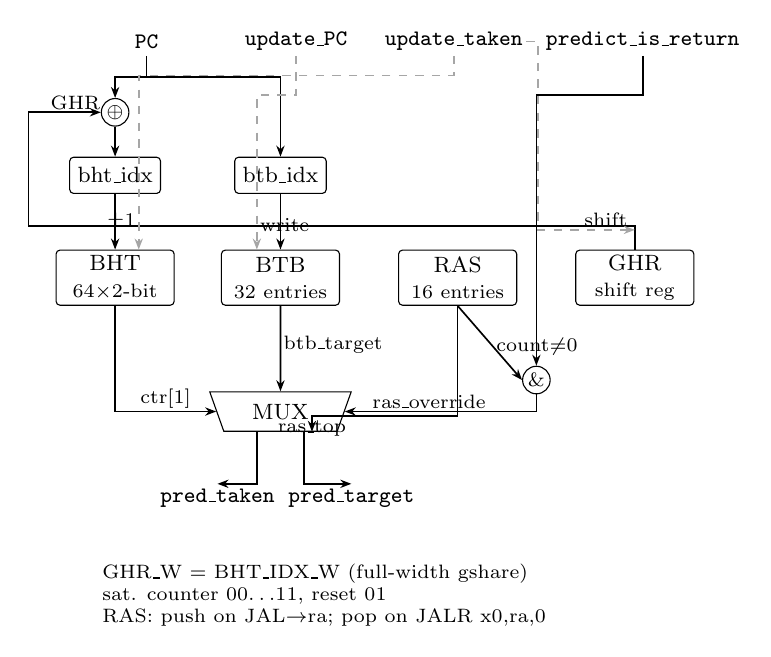
\begin{tikzpicture}[
    >={Stealth[length=1.4mm]},
    font=\footnotesize,
    box/.style    = {draw, rounded corners=0.5mm, minimum height=4.6mm,
                     minimum width=12mm, inner xsep=1mm, inner ysep=0.5mm,
                     align=center},
    store/.style  = {box, minimum width=15mm, minimum height=7mm},
    io/.style     = {minimum height=3.5mm, inner sep=0.4mm},
    op/.style     = {draw, circle, inner sep=0pt, minimum size=3.5mm,
                     font=\scriptsize},
    mux/.style    = {draw, trapezium, trapezium left angle=70,
                     trapezium right angle=70, trapezium stretches=true,
                     minimum width=18mm, minimum height=5mm,
                     shape border rotate=180, inner sep=0.4mm,
                     font=\footnotesize},
    pred/.style   = {->, semithick},
    upd/.style    = {->, dashed, draw=gray!70, semithick},
    lab/.style    = {font=\scriptsize, inner sep=0.3mm}
]

% ---------------- inputs (top row) ----------------
\node[io] (pc)   at (0.0, 0)  {\texttt{PC}};
\node[io] (upc)  at (1.9, 0)  {\texttt{update\_PC}};
\node[io] (utk)  at (3.9, 0)  {\texttt{update\_taken}};
\node[io] (pir)  at (6.3, 0)  {\texttt{predict\_is\_return}};

% ---------------- index logic row ----------------
\node[op]                       (xor)  at (-0.4,-0.9) {$\oplus$};
\node[box,minimum width=11mm]  (bhti) at (-0.4,-1.7) {bht\_idx};
\node[box,minimum width=11mm]  (btbi) at ( 1.7,-1.7) {btb\_idx};

% ---------------- state storage row ----------------
\node[store] (bht) at (-0.4,-3.0) {BHT\\\scriptsize 64$\times$2-bit};
\node[store] (btb) at ( 1.7,-3.0) {BTB\\\scriptsize 32 entries};
\node[store] (ras) at ( 3.95,-3.0) {RAS\\\scriptsize 16 entries};
\node[store] (ghr) at ( 6.2,-3.0) {GHR\\\scriptsize shift reg};

% ---------------- decision row ----------------
\node[op]   (and) at (4.95,-4.3) {\&};
\node[mux]  (mux) at (1.7,-4.7)  {MUX};

% ---------------- outputs ----------------
\node[io] (ptk) at (0.9,-5.8) {\texttt{pred\_taken}};
\node[io] (ptg) at (2.6,-5.8) {\texttt{pred\_target}};

% routing helper coordinates
\coordinate (ghr_route) at (-1.5,-0.9);

% ============= predict path (solid) =============
% PC stub -> branch point
\coordinate (pc_t) at (0.0,-0.45);
\draw[pred,-] (pc.south) -- (pc_t);
% PC stub -> XOR
\draw[pred] (pc_t) -| (xor.north);
% PC stub -> btb_idx
\draw[pred] (pc_t) -| (btbi.north);
% GHR -> (route up and over) -> XOR east input
\draw[pred] (ghr.north) -- ++(0,0.3) -| (ghr_route)
            -- node[lab,above,pos=0.65]{GHR} (xor.west);
% XOR -> bht_idx
\draw[pred] (xor.south) -- (bhti.north);
% indices -> storage
\draw[pred] (bhti.south) -- (bht.north);
\draw[pred] (btbi.south) -- (btb.north);

% BHT counter[1] -> MUX (west input)
\draw[pred] (bht.south) |- node[lab,pos=0.75,above]{ctr[1]} (mux.west);
% BTB target -> MUX (top / data input)
\draw[pred] (btb.south) -- node[lab,right,pos=0.45]{btb\_target} (mux.north);

% predict_is_return -> AND (right input via the top)
\draw[pred] (pir.south) -- ++(0,-0.5) -| (and.north);
% RAS count!=0 -> AND (left input)
\draw[pred] (ras.south) -- node[lab,right,pos=0.55]{count$\neq$0} (and.west);

% AND -> MUX select (right side as ras_override)
\draw[pred] (and.south) |- node[lab,pos=0.78,above]{ras\_override} (mux.east);

% RAS top -> MUX (alternate target along the bottom)
\draw[pred] (ras.south) -- ++(0,-1.4) -|
            node[lab,pos=0.55,below]{ras\_top}
            ([xshift=4mm]mux.south);

% MUX -> outputs
\draw[pred] ([xshift=-3mm]mux.south) |- (ptk.north);
\draw[pred] ([xshift= 3mm]mux.south) |- (ptg.north);

% ============= update path (dashed) =============
% update_taken -> BHT (saturating +/-1)
\draw[upd] (utk.south) -- ++(0,-0.25) -|
           node[lab,pos=0.92,left]{$\pm1$}
           ([xshift=3mm]bht.north);
% update_PC + target -> BTB write
\draw[upd] (upc.south) -- ++(0,-0.5) -|
           node[lab,pos=0.92,right]{write}
           ([xshift=-3mm]btb.north);
% update_taken -> GHR shift-in (feedback shift)
\draw[upd] (utk.east) -- ++(0.15,0) |-
           node[lab,pos=0.85,above]{shift}
           ([yshift=2.5mm]ghr.north);

% ============= annotations =============
\node[lab,align=left,anchor=north west] at (-0.6,-6.6) {%
    GHR\_W = BHT\_IDX\_W (full-width gshare)\\
    sat. counter $00\!\ldots\!11$, reset $01$\\
    RAS: push on JAL$\to$ra; pop on JALR x0,ra,0
};

\end{tikzpicture}

    \caption{Branch predictor combining gshare with a 16-entry Return Address Stack. The RAS overrides the BTB on returns; gshare's XOR of PC with the global history register de-aliases counters that bimodal would share.}
    \label{fig:predictor}
\end{figure}

\subsubsection{gshare}
% [Paste from draft.md §V.C.1]

\subsubsection{Return Address Stack}
% [Paste from draft.md §V.C.2]

\subsection{D-cache Enhancements}
% [Paste from draft.md §V.D]

% Figure 3 — D-cache organization
\begin{figure}[t]
    \centering
    % Figure 3 -- D-cache organization
% Left-to-right: address fields -> cache storage / comparators -> hit mux -> data out.
% Stream buffer drawn below as a parallel path to the memory bus (dashed wires).
% Uses only TikZ libraries already loaded in main.tex:
%   shapes.geometric, arrows.meta, positioning, fit
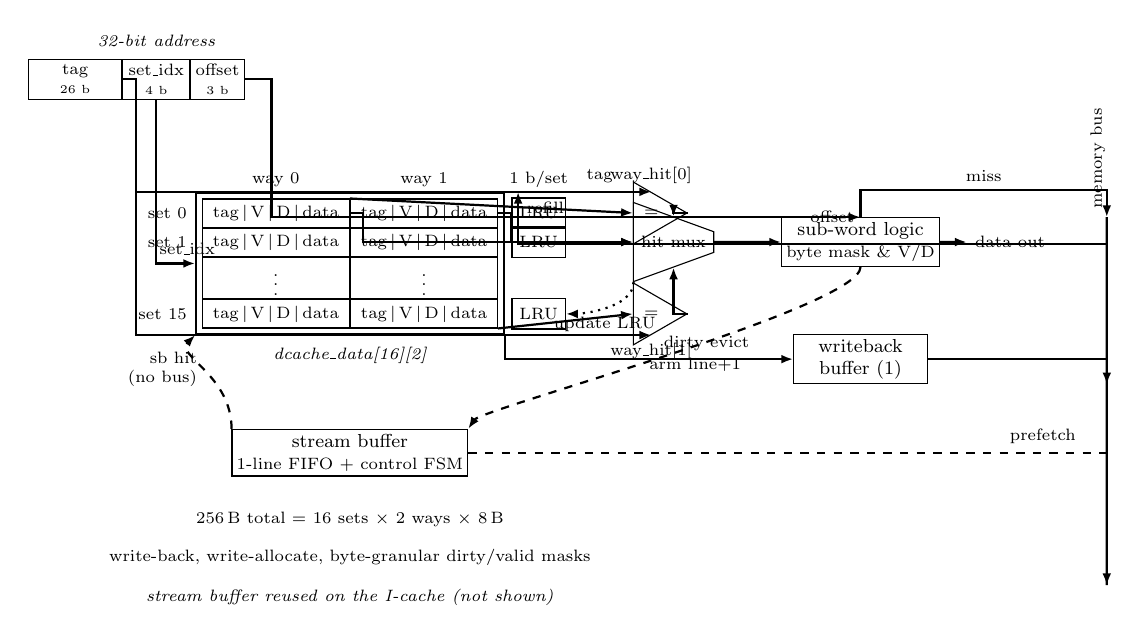
\begin{tikzpicture}[
    scale=0.85, transform shape,
    every node/.style={color=black, font=\footnotesize},
    box/.style={draw, rectangle, minimum height=6mm, minimum width=14mm,
                align=center, inner sep=2pt, color=black},
    smallbox/.style={draw, rectangle, minimum height=4.5mm, minimum width=8mm,
                     align=center, inner sep=1.5pt, font=\scriptsize, color=black},
    cell/.style={draw, rectangle, minimum height=4.2mm, minimum width=22mm,
                 align=center, inner sep=1.5pt, font=\scriptsize, color=black},
    fieldcell/.style={draw, rectangle, minimum height=6mm, align=center,
                      inner sep=1.5pt, font=\scriptsize, color=black},
    cmp/.style={draw, isosceles triangle, isosceles triangle apex angle=60,
                minimum height=8mm, inner sep=1pt, font=\scriptsize, color=black},
    mux/.style={draw, trapezium, trapezium left angle=70, trapezium right angle=70,
                minimum height=8mm, inner sep=1.5pt, shape border rotate=270,
                font=\scriptsize, color=black},
    annot/.style={font=\scriptsize, color=black, align=center},
    arrow/.style={-{Latex[length=1.5mm]}, color=black, thick},
    sideband/.style={-{Latex[length=1.5mm]}, color=black, dashed, thick},
    >={Latex[length=1.5mm]}
]

% =========================================================
% Address decomposition (top-left)
% =========================================================
\node[fieldcell, minimum width=14mm] (atag) at (0, 0) {tag\\\tiny 26 b};
\node[fieldcell, minimum width=10mm, right=0pt of atag] (aset) {set\_idx\\\tiny 4 b};
\node[fieldcell, minimum width=8mm,  right=0pt of aset] (aoff) {offset\\\tiny 3 b};
\node[annot, above=0.5mm of aset.north] {\itshape 32-bit address};

% =========================================================
% Cache storage grid (16 sets x 2 ways), abbreviated rows
% Anchored relative to the address fields by absolute coordinates
% =========================================================
\node[cell] (w0r0)  at (3.0, -2.0) {tag\,\textbar\,V\,\textbar\,D\,\textbar\,data};
\node[cell, below=0pt of w0r0]  (w0r1)   {tag\,\textbar\,V\,\textbar\,D\,\textbar\,data};
\node[cell, below=0pt of w0r1]  (w0dots) {\vdots};
\node[cell, below=0pt of w0dots](w0r15)  {tag\,\textbar\,V\,\textbar\,D\,\textbar\,data};

\node[cell, right=0pt of w0r0]   (w1r0)   {tag\,\textbar\,V\,\textbar\,D\,\textbar\,data};
\node[cell, right=0pt of w0r1]   (w1r1)   {tag\,\textbar\,V\,\textbar\,D\,\textbar\,data};
\node[cell, right=0pt of w0dots] (w1dots) {\vdots};
\node[cell, right=0pt of w0r15]  (w1r15)  {tag\,\textbar\,V\,\textbar\,D\,\textbar\,data};

% Column headers
\node[annot, above=0.5mm of w0r0] {way 0};
\node[annot, above=0.5mm of w1r0] {way 1};

% Set-row labels on the far left of the grid
\node[annot, left=1mm of w0r0]  {set 0};
\node[annot, left=1mm of w0r1]  {set 1};
\node[annot, left=1mm of w0r15] {set 15};

% Group label below the grid
\node[draw, thick, fit=(w0r0) (w1r15), inner sep=2pt] (gridbox) {};
\node[annot, below=0.5mm of gridbox.south]
    {\itshape dcache\_data[16][2]};

% LRU column (one bit per set, just to the right of the grid)
\node[smallbox, right=2mm of w1r0,  minimum width=8mm] (lru0)  {LRU};
\node[smallbox, right=2mm of w1r1,  minimum width=8mm] (lru1)  {LRU};
\node[smallbox, right=2mm of w1r15, minimum width=8mm] (lru15) {LRU};
\node[annot, above=0.2mm of lru0.north] {1 b/set};

% =========================================================
% Comparators (one per way)
% =========================================================
\node[cmp, right=10mm of lru0]  (cmp0) {=};
\node[cmp, right=10mm of lru15] (cmp1) {=};
\node[annot, above=0pt of cmp0.north] {way\_hit[0]};
\node[annot, below=0pt of cmp1.south] {way\_hit[1]};

% =========================================================
% Hit mux + sub-word logic + data out
% =========================================================
\node[mux, right=10mm of lru1, minimum height=12mm, minimum width=10mm] (hitmux) {hit mux};
\node[box, right=10mm of hitmux, minimum width=20mm] (subw)
    {sub-word logic\\\scriptsize byte mask \& V/D};
\node[annot, right=4mm of subw] (dout) {data out};

% =========================================================
% Writeback buffer (below subword block)
% =========================================================
\node[box, below=10mm of subw, minimum width=20mm] (wbuf)
    {writeback\\buffer (1)};

% =========================================================
% Memory bus (vertical spine on far right)
% =========================================================
\coordinate (busTop) at ([xshift=8mm] dout.east  |- subw.north);
\coordinate (busBot) at ([xshift=8mm] dout.east  |- wbuf.south);
\coordinate (busFar) at ([yshift=-30mm] busBot);
\draw[thick] (busTop) -- (busFar);
\node[annot, right=1mm of busTop, rotate=90, anchor=south west] {memory bus};

% =========================================================
% Stream buffer (below the cache, parallel path to memory bus)
% =========================================================
\node[box, below=14mm of gridbox.south, minimum width=34mm] (sbuf)
    {stream buffer\\\scriptsize 1-line FIFO + control FSM};

% =========================================================
% Arrows -- address fanout
% =========================================================
% set_idx -> grid (left edge)
\draw[arrow] (aset.south) |- node[pos=0.9, above, font=\scriptsize] {set\_idx} (gridbox.west);
% tag -> both comparators (right input)
\draw[arrow] (atag.east) -- ([xshift=2mm] atag.east)
    |- node[pos=0.95, above, font=\scriptsize] {tag} (cmp0.north);
\draw[arrow] (atag.east) -- ([xshift=2mm] atag.east)
    |- (cmp1.south);
% offset -> sub-word logic
\draw[arrow] (aoff.east) -- ([xshift=4mm] aoff.east)
    |- node[pos=0.95, right, font=\scriptsize] {offset} (subw.north);

% =========================================================
% Arrows -- way storage to comparators / hit mux
% =========================================================
% way[i].tag -> comparator[i]
\draw[arrow] (w0r0.north east) -- (cmp0.west);
\draw[arrow] (w1r15.south east) -- (cmp1.west);

% Comparator outputs -> hit mux (selects)
\draw[arrow] (cmp0.east) -| (hitmux.north);
\draw[arrow] (cmp1.east) -| (hitmux.south);

% Way data -> hit mux (data inputs)
\draw[arrow] (w0r0.east) -- ([xshift=2mm] w0r0.east) |- (hitmux.west);
\draw[arrow] (w1r0.east) -- ([xshift=2mm] w1r0.east) |- (hitmux.west);

% Hit mux -> sub-word -> data out
\draw[arrow] (hitmux.east) -- (subw.west);
\draw[arrow] (subw.east) -- (dout.west);

% LRU update on hit (annotation arrow)
\draw[arrow, dotted] (hitmux.south west) .. controls +(0,-4mm) and +(2mm,0) ..
    node[below, font=\scriptsize, pos=0.5] {update LRU} (lru15.east);

% =========================================================
% Memory traffic -- solid (demand) arrows
% =========================================================
% Miss request: from sub-word logic up onto bus
\draw[arrow] (subw.north) -- ([yshift=4mm] subw.north) -| (busTop)
    node[pos=0.25, above, font=\scriptsize] {miss};
% Refill (LRU pick): from bus back into the grid
\draw[arrow] ([yshift=-4mm] busTop) -| ([xshift=2mm] gridbox.north east)
    node[pos=0.85, right, font=\scriptsize] {refill};
% Dirty eviction -> writeback buffer -> bus
\draw[arrow] (gridbox.south east) |- (wbuf.west)
    node[pos=0.85, above, font=\scriptsize] {dirty evict};
\draw[arrow] (wbuf.east) -| (busBot);

% =========================================================
% Stream-buffer (speculative) -- dashed arrows
% =========================================================
% Arm stream buffer for line+1 after a miss
\draw[sideband] (subw.south) .. controls +(0,-6mm) and +(2mm,3mm) ..
    node[right, font=\scriptsize, pos=0.55] {arm line+1} (sbuf.north east);
% Stream buffer <-> memory bus (prefetch fill)
\draw[sideband] (sbuf.east) -| (busFar)
    node[pos=0.45, above, font=\scriptsize] {prefetch};
% Stream-buffer hit absorbs subsequent miss into the cache without bus traffic
\draw[sideband] (sbuf.north west) .. controls +(0,8mm) and +(-3mm,-3mm) ..
    node[left, font=\scriptsize, pos=0.5, align=right] {sb hit\\(no bus)} (gridbox.south west);

% =========================================================
% Annotations (bottom of figure)
% =========================================================
\node[annot, below=4mm of sbuf] (aA)
    {256\,B total = 16 sets $\times$ 2 ways $\times$ 8\,B};
\node[annot, below=1mm of aA] (aB)
    {write-back, write-allocate, byte-granular dirty/valid masks};
\node[annot, below=1mm of aB]
    {\itshape stream buffer reused on the I-cache (not shown)};

\end{tikzpicture}

    \caption{Two-way set-associative D-cache with one-line stream buffer. The stream buffer arms after every demand miss and absorbs sequential line-walks without round-tripping to memory.}
    \label{fig:dcache}
\end{figure}

\subsubsection{2-way set-associative D-cache}
% [Paste from draft.md §V.D.1]

\subsubsection{Next-Line Prefetch / Stream Buffer}
% [Paste from draft.md §V.D.2]

\subsection{Store-to-Load Forwarding}
% [Paste from draft.md §V.E]

% Figure 4 — Store-to-load forwarding lanes
\begin{figure}[t]
    \centering
    % Figure 4 — Store-to-load forwarding lanes
% Left: LSQ as a circular buffer (head/tail, slot fields).
% Middle: per-load forwarding cone (addr compare, byte-mask intersect, priority encoder).
% Right: +1-cycle defer latch (dashed) feeding a CDB output port.
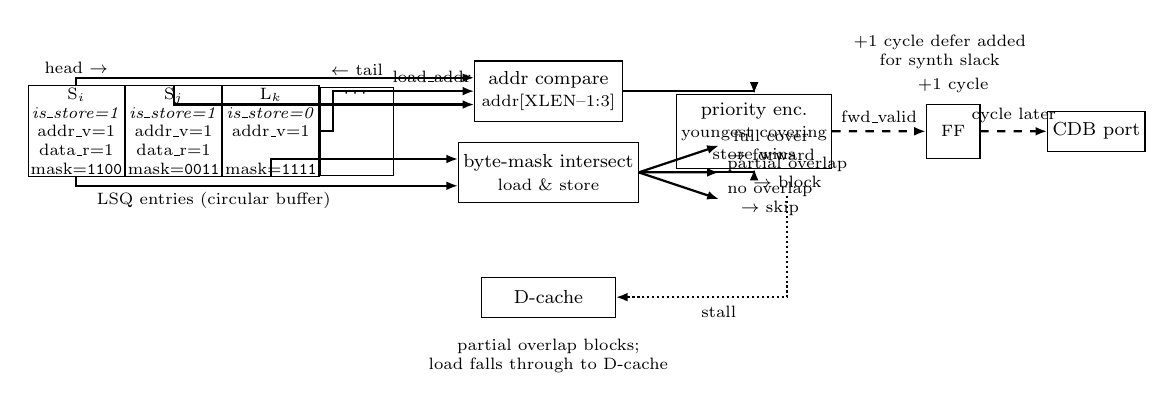
\begin{tikzpicture}[
    scale=0.85, transform shape,
    every node/.style={color=black, font=\footnotesize},
    box/.style={draw, rectangle, minimum height=6mm, minimum width=14mm,
                align=center, inner sep=2pt, color=black},
    slot/.style={draw, rectangle, minimum height=11mm, minimum width=11mm,
                 align=center, inner sep=1pt, font=\scriptsize, color=black},
    ff/.style={draw, rectangle, minimum height=8mm, minimum width=8mm,
               align=center, inner sep=1pt, font=\scriptsize, color=black},
    annot/.style={font=\scriptsize, color=black, align=center},
    arrow/.style={-{Latex[length=1.5mm]}, color=black, thick},
    defer/.style={-{Latex[length=1.5mm]}, color=black, dashed, thick},
    stalled/.style={-{Latex[length=1.5mm]}, color=black, thick, densely dotted},
    >={Latex[length=1.5mm]}
]

% =========================================================
% LEFT: LSQ as a row of circular-buffer slots
% =========================================================
\node[slot] (s0) at (0, 0)
    {S$_{i}$\\\textit{is\_store=1}\\addr\_v=1\\data\_r=1\\mask=\texttt{1100}};
\node[slot, right=0mm of s0] (s1)
    {S$_{j}$\\\textit{is\_store=1}\\addr\_v=1\\data\_r=1\\mask=\texttt{0011}};
\node[slot, right=0mm of s1] (sL)
    {L$_{k}$\\\textit{is\_store=0}\\addr\_v=1\\\,\\mask=\texttt{1111}};
\node[slot, right=0mm of sL] (s3)
    {$\cdots$\\\,\\\,\\\,\\\,};

% head / tail pointers
\node[annot, above=0.5mm of s0] {head $\rightarrow$};
\node[annot, above=0.5mm of s3] {$\leftarrow$ tail};

% Group label for the LSQ
\node[annot, below=1mm of s1, xshift=6mm] {LSQ entries (circular buffer)};

% =========================================================
% MIDDLE: per-load forwarding cone
% =========================================================
% Address comparator
\node[box, right=12mm of s3, yshift=6mm,
      minimum width=22mm, minimum height=9mm] (cmp)
    {addr compare\\\scriptsize{addr[XLEN--1:3]}};

% Byte-mask intersect
\node[box, below=3mm of cmp, minimum width=22mm, minimum height=9mm] (mask)
    {byte-mask intersect\\\scriptsize{load \& store}};

% Priority encoder: youngest covering store wins
\node[box, right=8mm of cmp, yshift=-6mm,
      minimum width=18mm, minimum height=11mm] (pe)
    {priority enc.\\\scriptsize{youngest covering}\\\scriptsize{store wins}};

% Outcome labels off the byte-mask block
\node[annot, right=12mm of mask, yshift=4mm]   (full)  {full cover\\$\rightarrow$ forward};
\node[annot, right=12mm of mask]               (part)  {partial overlap\\$\rightarrow$ block};
\node[annot, right=12mm of mask, yshift=-4mm]  (none)  {no overlap\\$\rightarrow$ skip};

% =========================================================
% RIGHT: +1-cycle defer latch and CDB output port
% =========================================================
\node[ff, right=14mm of pe] (latch) {FF};
\node[annot, above=0.5mm of latch] {+1 cycle};

\node[box, right=10mm of latch, minimum width=14mm] (cdb) {CDB port};

% =========================================================
% ARROWS
% =========================================================
% load_addr fanout from load slot to comparator
\draw[arrow] (sL.east) -- ++(2mm,0) |- (cmp.west)
    node[pos=0.85, above, font=\scriptsize] {load\_addr};
% older store addresses to comparator
\draw[arrow] (s0.north) |- ([yshift=2mm]cmp.west);
\draw[arrow] (s1.north) |- ([yshift=-2mm]cmp.west);

% load + store masks into the byte-mask intersect
\draw[arrow] (sL.south) |- ([yshift=2mm]mask.west);
\draw[arrow] (s0.south) |- ([yshift=-2mm]mask.west);

% comparator + mask outcomes feed priority encoder
\draw[arrow] (cmp.east) -| (pe.north);
\draw[arrow] (mask.east) -| (pe.south);

% outcome callouts (full / partial / no-overlap) drawn off the mask block
\draw[arrow] (mask.east) -- (full.west);
\draw[arrow] (mask.east) -- (part.west);
\draw[arrow] (mask.east) -- (none.west);

% forward valid -> latch -> CDB (dashed +1-cycle defer lane)
\draw[defer] (pe.east) -- node[above, font=\scriptsize] {fwd\_valid} (latch.west);
\draw[defer] (latch.east) -- node[above, font=\scriptsize] {cycle later} (cdb.west);

% Block path: partial overlap -> load falls through to the D-cache (stalled edge)
\node[box, below=11mm of mask, minimum width=20mm] (dcache) {D-cache};
\draw[stalled] (part.south) |- (dcache.east)
    node[pos=0.7, below, font=\scriptsize] {stall};

% =========================================================
% ANNOTATIONS
% =========================================================
\node[annot, above=4mm of latch, xshift=-2mm]
    {+1 cycle defer added\\for synth slack};

\node[annot, below=2mm of dcache]
    {partial overlap blocks;\\load falls through to D-cache};

\end{tikzpicture}

    \caption{Store-to-load forwarding. A load at the LSQ head compares against older un-committed stores; a clean byte-cover match forwards the value through a one-cycle latch onto the CDB.}
    \label{fig:stlf}
\end{figure}

\section{Verification and Testing Methodology}
% [Paste from draft.md §VI]

\section{Performance Evaluation and Analysis}
% [Paste from draft.md §VII]

% Table II — Per-program performance, representative subset (placeholder; see Task 25)
% [TABLE II goes here — migrated in Task 25]

% Table III — Per-program performance, full 34-row continuation (placeholder; see Task 25)
% [TABLE III goes here — migrated in Task 25]

% Table IV — Per-feature attribution (placeholder; see Task 25)
% [TABLE IV goes here — migrated in Task 25]

% Table V — Per-module synthesis slack (placeholder; see Task 25)
% [TABLE V goes here — migrated in Task 25]

\section{Discussion: Limitations and Future Work}
% [Paste from draft.md §VIII]

\section{Conclusion}
% [Paste from draft.md §IX]

\bibliographystyle{IEEEtran}
\bibliography{refs}

\end{document}
